\section{Módulo textual: índice invertido en disco}
\label{sec:textual}

\subsection{Pipeline léxico y SPIMI}

El preprocesamiento (\code{backend/text/preprocess.py}) tokeniza con una expresión
regular de letras Unicode, pasa a minúsculas, elimina las stopwords de NLTK en
español e inglés y aplica el stemmer Snowball del idioma detectado (el que más
stopwords aporta al documento; la consulta pasa por los dos stemmers). Cada término
se corta a 24 bytes porque el vocabulario lo guarda en un \code{CHAR} de ancho fijo.

La construcción es SPIMI (\code{spimi.py}): una pasada sobre los documentos acumula
término $\to$ postings en RAM hasta un presupuesto de postings, vuelca cada bloque
ordenado a disco y al final hace un merge de $k$ vías con un heap, leyendo una
página por bloque. Como el merge es estable y la tabla se recorre en orden de RID,
cada lista de posteo queda ordenada por RID sin reordenarla.

\subsection{Diseño en disco}

Un índice \code{INVERTED} sobre la columna de una tabla son cuatro archivos paginados
por el \code{Pager}:

\begin{table}[H]
\centering\small
\begin{tabularx}{\textwidth}{lY}
\toprule
Archivo & Contenido \\
\midrule
\code{<t>\_\_<idx>.inv.meta} & cabecera autodescriptiva: la columna indexada, el ranking por defecto (\code{user\_a}) y si el índice quedó desactualizado (\code{user\_b}) \\
\code{...inv.vocab.dic} & diccionario: un árbol B+ del Proyecto~1 con clave \code{CHAR(24)} (el término $t$) y valor $\langle$offset de la lista en \code{postings.inv}, $df_t\rangle$; como cada documento aparece una vez por término, el largo de la lista de posteo es $df_t$ \\
\code{...inv.postings.inv} & listas de posteo: un arreglo contiguo de registros $\langle$page, slot, $tf_{t,d}$, $|d|\rangle$ de 16 bytes (252 por página), con las listas una detrás de otra y ordenadas por RID; $N$ y $\sum|d|$ van en la cabecera \\
\code{...inv.norms.dat} & la norma euclidiana $\|\vec d\|_2$ de cada documento, precalculada para el coseno \\
\bottomrule
\end{tabularx}
\caption{Archivos del índice invertido.}
\end{table}

\begin{figure}[H]
\centering
\begin{tikzpicture}[
  pg/.style={draw, rounded corners=1pt, minimum width=1.5cm, minimum height=0.85cm,
             font=\scriptsize, align=center},
  >={Stealth[length=2mm]}, node distance=0.22cm]
  \node[font=\footnotesize\bfseries, anchor=west] at (-0.8,3.1) {\texttt{vocab.dic} (B+): término $\to$ (offset, $df$)};
  \node[pg, fill=blue!10] (r) at (3.2,2.35) {raíz};
  \node[pg, fill=blue!6] (h1) at (0.6,1.4) {hoja\\\texttt{guerr}: (812, 37)};
  \node[pg, fill=blue!6, right=of h1] (h2) {hoja\\\texttt{histori}: (849, 61)};
  \node[right=of h2] (hd) {$\cdots$};
  \draw[->] (r) -- (h1.north);
  \draw[->] (r) -- (h2.north);
  \draw[->, dashed] (h1) -- (h2);

  \node[font=\footnotesize\bfseries, anchor=west] at (-0.8,-1.2) {\texttt{postings.inv}: un arreglo contiguo, listas ordenadas por RID};
  \node[pg, fill=gray!15] (p0) at (0,-0.4) {pág.\ 0\\$N$, $\sum|d|$};
  \node[pg, fill=orange!18, right=of p0] (p1) {pág.\ 1};
  \node[right=of p1] (pd) {$\cdots$};
  \node[pg, fill=orange!18, right=of pd] (p4) {pág.\ 4\\pos.\ 812..};
  \node[pg, fill=orange!18, right=of p4] (p5) {pág.\ 4--5\\pos.\ 849..};
  \draw[->, blue!60!black] (h1.south) .. controls +(0,-0.7) and +(0,0.7) .. (p4.north);
  \draw[->, blue!60!black] (h2.south) .. controls +(0,-0.7) and +(0,0.7) .. (p5.north);
\end{tikzpicture}
\caption{Diseño físico del índice invertido. Ubicar un término cuesta la altura del B+;
leer su lista cuesta las páginas que ocupa ($\lceil df/252\rceil$, a veces una más si la
lista cruza un borde de página). Las listas van seguidas porque la mayoría de los términos
aparece en un solo documento: darle a cada lista su propia página desperdiciaría casi todo
el archivo.}
\label{fig:inv-disco}
\end{figure}

El RID de cada posting es el $\langle$page, slot$\rangle$ de la fila. En el Sequential
File el área de overflow se marca con un bit alto de \code{page}, de modo que el orden de
los RID coincide con el del recorrido de la tabla (área principal y luego overflow) y las
mezclas booleanas siguen funcionando.

\subsection{Recuperación booleana y ranking}

\paragraph{Consultas booleanas en $O(n+m)$.} \code{backend/text/boolean.py} implementa la
intersección (\code{AND}), la unión (\code{OR}) y la diferencia (\code{AND-NOT}) con la
mezcla de dos punteros sobre listas ordenadas: cada lista se recorre una sola vez. La
consulta se parsea con la precedencia usual (\code{NOT} > \code{AND} > \code{OR}),
paréntesis y \code{AND} implícito entre palabras seguidas. Un \code{AND} intersecta primero
de la lista más corta a la más larga, para que el resultado intermedio nunca crezca, y
recién después resta las listas negadas. Un \code{NOT} necesita un término positivo al lado
(\code{a AND NOT b}): el complemento de una lista no se puede recorrer en el índice. Una
palabra que es stopword no filtra.

\paragraph{Ranking.} Sobre los mismos archivos conviven dos funciones de score. TF-IDF con
similitud de coseno, como pide el enunciado:
\[
w_{t,d} = (1+\log_{10} tf_{t,d})\cdot\log_{10}\frac{N}{df_t}
\qquad
\text{score}(q,d)=\frac{\sum_{t\in q} w_{t,q}\,w_{t,d}}{\|\vec q\|_2\,\|\vec d\|_2}
\]
y BM25, que el enunciado admite como alternativa. Solo se leen las listas de los términos
de la consulta; los productos parciales se acumulan en un diccionario y el top-$k$ sale de
un heap. Cada lista se lee una vez aunque el término participe a la vez del filtro booleano
y del score.

\subsection{Integración con SQL}

\begin{lstlisting}
CREATE INDEX idx_texto ON documentos (texto) USING INVERTED WITH (scoring = 'TFIDF_COSINE');
SELECT id, titulo, COSINE_SCORE() AS relevancia FROM documentos
WHERE texto MATCH 'aprendizaje AND profundo AND NOT basico' AND anio >= 2010
ORDER BY relevancia DESC LIMIT 10;
\end{lstlisting}

Una consulta con operadores (\code{AND}, \code{OR}, \code{NOT}, paréntesis) es booleana: el
resultado son los documentos que la cumplen, ordenados por relevancia. Sin operadores es
una consulta de ranking: las palabras se combinan con \code{OR} y el orden lo da el score.
\code{COSINE\_SCORE()} y \code{BM25\_SCORE()} eligen la función de score de la consulta; sin
ellas se usa la del índice (\code{WITH (scoring = ...)}).

El executor resuelve \code{MATCH} con un esquema de filtro y refinamiento
(\code{InvertedIndexScan}). El índice entrega los documentos que cumplen y su score leyendo
solo el vocabulario y las listas de la consulta, sin tocar la tabla. Después se leen las
filas candidatas por RID en orden de relevancia, se aplican los demás predicados del
\code{WHERE} y, con un \code{LIMIT} sobre el score, la lectura para al juntar $k$ filas. Sin
índice invertido la misma consulta se resuelve con un Full Text Scan (\code{TextSeqScan})
que lee toda la tabla y preprocesa cada documento; las dos rutas devuelven exactamente el
mismo resultado, que es lo que verifican los tests. Si además la consulta se ordena por una
distancia vectorial, los candidatos del texto alimentan un k-NN exacto
(\code{TextPreFilter}): texto, predicados relacionales y similitud vectorial en una sola
consulta. El plan reporta el modo, los términos, las listas y postings leídos, las filas
traídas de la tabla y el I/O del índice y de la tabla por separado.

\paragraph{Mantenimiento.} SPIMI construye el índice de una vez. Un \code{INSERT}, un
\code{DELETE} o una reorganización solo lo marcan como desactualizado (escribir la cabecera
cuesta una página) y la siguiente consulta \code{MATCH} lo reconstruye antes de usarlo; el
plan lo indica y el costo aparece como escrituras del índice. Es el modelo de reindexación
por lotes de los motores de búsqueda: mantener listas comprimidas y contiguas en cada
inserción obligaría a reescribirlas.

\subsection{Experimento 6: índice invertido vs.\ Full Text Scan vs.\ GIN}

\paragraph{Metodología.} Corpus de 100\,000 artículos de Wikipedia (50\,000 en español y
50\,000 en inglés, los primeros 1000 bytes de cada uno), leídos del primer archivo parquet
de cada idioma con \code{backend/text/wikipedia.py}. Fuente: volcado
\code{wikimedia/wikipedia} 20231101 (Hugging Face), licencia CC BY-SA 4.0. Todo corre por SQL a través del executor
(\code{backend/benchmarks/experiment6.py}), con páginas de 4\,KB y sin buffer pool. La
referencia externa es PostgreSQL~16 en un contenedor, con una columna
\code{tsvector} generada con el diccionario del idioma de cada documento y un índice GIN
sobre ella; su I/O se mide con \code{EXPLAIN (ANALYZE, BUFFERS)} (bloques compartidos leídos
o encontrados en caché, de 8\,KB). Las consultas salen del propio corpus: las palabras de
un \code{AND} se toman de un mismo documento, para que el resultado no quede vacío, y la
palabra negada de un \code{AND-NOT} es una palabra frecuente que ese documento no tiene. Se
usaron 20 consultas por celda para el índice y GIN y 2 para el Full Text Scan, cuya
latencia casi no varía entre consultas.

\paragraph{Construcción.}

\begin{table}[H]
\centering\small
\begin{tabular}{rrrrrr}
\toprule
Documentos & \multicolumn{2}{c}{Índice invertido} & \multicolumn{2}{c}{GIN (PostgreSQL)} & Escrituras \\
 & tiempo (s) & tamaño (MB) & tiempo (s) & tamaño (MB) & del índice \\
\midrule
1\,000 & 11,3 & 1,9 & 0,07 & 1,1 & 14\,618 \\
10\,000 & 93,6 & 13,8 & 0,56 & 6,4 & 68\,813 \\
25\,000 & 231,1 & 31,9 & 1,60 & 13,8 & 136\,513 \\
50\,000 & 458,7 & 61,8 & 3,23 & 25,5 & 234\,516 \\
100\,000 & 1\,052,8 & 123,6 & 8,60 & 43,4 & 468\,239 \\
\bottomrule
\end{tabular}
\caption{Experimento 6a (\code{exp6\_construccion.csv}): construcción del índice invertido (vocabulario + postings + normas) y del GIN.}
\end{table}

\begin{figure}[H]
\centering
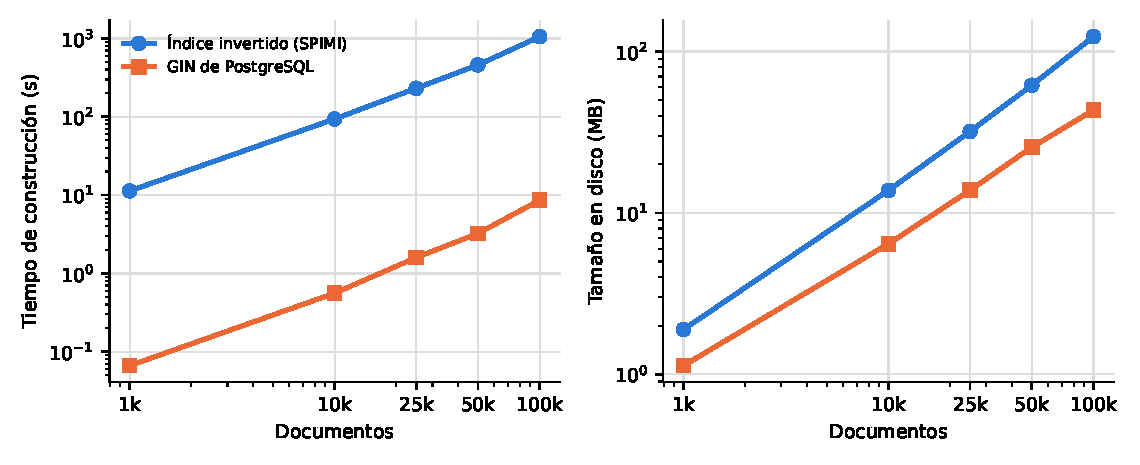
\includegraphics[width=0.95\textwidth]{exp6_construccion}
\caption{Tiempo de construcción y tamaño en disco al crecer el corpus (escala log-log). El índice invertido crece linealmente en tamaño; el GIN crece más lento porque comprime mejor las listas largas.}
\end{figure}

El nuestro crece linealmente: unos 10,5\,ms y 1,2\,KB por documento con 100\,000
documentos. El GIN cuesta 0,09\,ms y 0,4\,KB por documento, y su tamaño crece más lento
que el corpus (de 1,1 a 0,4\,KB por documento) porque las listas largas se comprimen
mejor. La diferencia de tamaño es de diseño: nuestros postings son
registros fijos de 16 bytes sin comprimir que guardan además $tf$ y $|d|$ (los necesita el
ranking sin tocar la tabla), el vocabulario usa claves \code{CHAR(24)} de ancho fijo y hay
un archivo de normas; el GIN comprime las listas (deltas codificados en bytes variables) y
no guarda frecuencias. La diferencia de tiempo (unas 120 veces) viene de que el vocabulario se
arma insertando término por término en el B+ del Proyecto~1 desde Python (468\,239
escrituras de bloque para 100\,000 documentos), mientras que PostgreSQL ordena en memoria y
construye el árbol de abajo hacia arriba en C.

\paragraph{Consultas.}

\begin{table}[H]
\centering\small
\begin{tabular}{rlrrrrrrr}
\toprule
 & & \multicolumn{2}{c}{Índice invertido} & \multicolumn{2}{c}{GIN} & \multicolumn{2}{c}{Full Text Scan} & \\
Términos & Operación & ms & bloques & ms & bloques & ms & bloques & coinciden \\
\midrule
1 & AND (un término) & 273,7 & 4\,155 & 60,3 & 11\,905 & 262\,794 & 25\,000 & 4\,133 \\
1 & Top-10 & 20,5 & 45 & 42,3 & 5\,257 & 283\,671 & 25\,000 & 2\,142 \\
3 & AND & 23,0 & 87 & 0,3 & 40 & 280\,511 & 25\,000 & 20 \\
3 & AND-NOT & 53,0 & 268 & 3,5 & 197 & 265\,128 & 25\,000 & 191 \\
3 & OR & 80,2 & 1\,728 & 14,7 & 1\,388 & 253\,852 & 25\,000 & 1\,682 \\
3 & Top-10 & 29,9 & 72 & 146,0 & 14\,871 & 304\,178 & 25\,000 & 5\,723 \\
5 & AND & 39,8 & 105 & 1,6 & 41 & 261\,475 & 25\,000 & 1 \\
5 & AND-NOT & 44,3 & 122 & 1,9 & 50 & 258\,904 & 25\,000 & 11 \\
5 & OR & 55,0 & 1\,022 & 2,8 & 829 & 253\,416 & 25\,000 & 969 \\
5 & Top-10 & 47,7 & 102 & 389,2 & 67\,941 & 252\,532 & 25\,000 & 9\,727 \\
\bottomrule
\end{tabular}
\caption{Experimento 6b (\code{exp6\_consultas.csv}), $N=100\,000$: latencia y bloques por consulta. ``Coinciden'' es el promedio de documentos que cumplen el \code{MATCH} con el índice. Bloques de 4\,KB en nuestro motor y de 8\,KB en PostgreSQL.}
\end{table}

\begin{figure}[H]
\centering
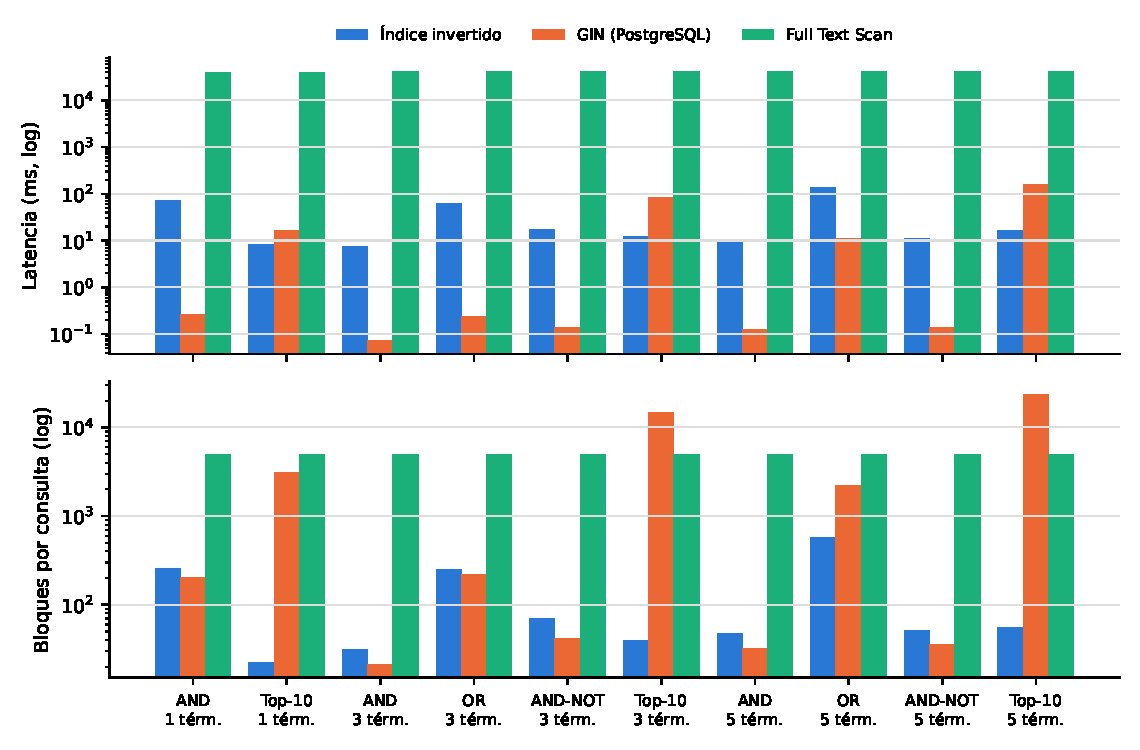
\includegraphics[width=0.95\textwidth]{exp6_consultas}
\caption{Latencia y bloques por consulta (escala logarítmica) de las tres rutas.}
\end{figure}

\paragraph{Análisis.} El Full Text Scan cuesta lo mismo para cualquier consulta: lee las
25\,000 páginas de la tabla y vuelve a preprocesar los 100\,000 documentos (tokenizar, quitar
stopwords, aplicar el stemmer y calcular normas), de 253 a 304 segundos. El índice resuelve las
mismas consultas entre 960 y 13\,800 veces más rápido y con 6 a 560 veces menos bloques. La
parte que lee el índice en sí es pequeña (de 22 a 111 bloques: la altura del B+ más las
páginas de las listas de la consulta); el resto son las filas del resultado traídas de la
tabla, una por documento, porque el \code{SELECT} pide columnas de la tabla. Por eso en
las consultas booleanas los bloques crecen con el número de documentos que cumplen (un
\code{AND} de un solo término trae 4\,133 filas) y, salvo en ese caso, quedan cerca de los
del GIN, que también debe visitar el heap por cada fila.

En las consultas de ranking Top-10 el índice gana a GIN en bloques (de 45 a 102 frente a
5\,257 a 67\,941) y en tiempo (de 20 a 48\,ms frente a 42 a 389\,ms). El score sale entero de
los postings ($tf$ y $|d|$) y de las normas, sin tocar la tabla, así que solo se leen las
10 filas del resultado. \code{ts\_rank} de PostgreSQL, en cambio, necesita el
\code{tsvector} de cada documento que cumple, que vive en el heap: su costo crece con los
5\,723 o 9\,727 documentos que coinciden y no con $k$. Guardar $tf$ y $|d|$ en cada posting
cuesta casi el triple de espacio que el GIN (123,6 frente a 43,4\,MB), y esta es la consulta
donde se recupera.

En las consultas booleanas el GIN es mucho más rápido (de 0,3 a 60\,ms frente a 23 a 274\,ms)
con un número parecido de bloques. Esa diferencia no es de I/O sino de implementación: C
contra Python, y el buffer pool de PostgreSQL contra nuestro motor sin caché, donde cada
acceso cuenta como lectura a propósito para que el \code{DiskCounter} mida la estructura y
no la caché.

Los resultados coinciden: para cada consulta el índice y el Full Text Scan devolvieron
exactamente los mismos documentos (el script lo verifica), y con GIN el número de
documentos difiere en menos de 1\,\% en casi todas las celdas (5\,\% en el Top-10 de un
término), por las pequeñas diferencias entre sus listas de
stopwords y diccionarios y los nuestros.
